\documentclass{article}
\usepackage{xstring}
\usepackage{tikz}
\usetikzlibrary{calc}
\usetikzlibrary{calc,chains,scopes,shapes.misc,backgrounds}
\pgfdeclarelayer{background}
\pgfdeclarelayer{foreground}

\pgfsetlayers{background,main,foreground}%,foreforeground}

% set up externalization
\usetikzlibrary{external}
\tikzset{external/system call={latex \tikzexternalcheckshellescape -halt-on-error
-interaction=batchmode -jobname "\image" "\texsource";
dvips -o "\image".ps "\image".dvi;
ps2eps "\image.ps"}}
\tikzexternalize



%    Column B contains numbers 1 - 15
%    Column I contains numbers 16 - 30
%    Column N contains numbers 31 - 45
%    Column G contains numbers 46 - 60
%    Column O contains numbers 61 - 75

\def\NumOfColumns{5}%
\def\Sequence{1/A/1/15, 2/B/16/30, 3/C/31/45, 4/D/46/60, 5/E/61/71}%

\newcommand{\Size}{2cm}
\tikzset{Square/.style={
    inner sep=0pt,
    text width=\Size, 
    minimum size=\Size,
    draw=black,
    fill=yellow!20,
    align=center,
    }
}

\begin{document}
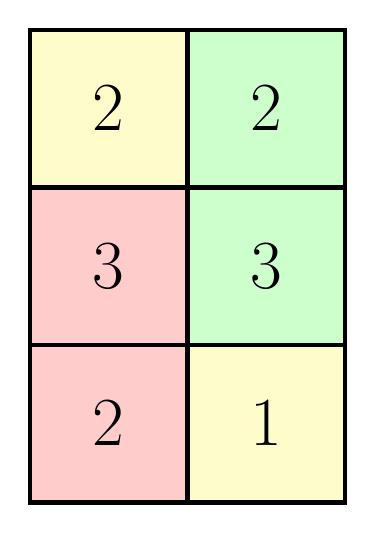
\begin{tikzpicture}[draw=black, ultra thick, x=\Size,y=\Size]
    \pgfmathsetmacro{\col}{1}; \pgfmathsetmacro{\row}{1};
    \node [Square] at ($(\col,-\row)-(0.5,0.5)$) {\Huge 2};
    \pgfmathsetmacro{\col}{1}; \pgfmathsetmacro{\row}{2};
    \node [Square,fill=red!20] at ($(\col,-\row)-(0.5,0.5)$) {\Huge 3};
    \pgfmathsetmacro{\col}{1}; \pgfmathsetmacro{\row}{3};
    \node [Square,fill=red!20] at ($(\col,-\row)-(0.5,0.5)$) {\Huge 2};
    \pgfmathsetmacro{\col}{2}; \pgfmathsetmacro{\row}{1};
    \node [Square,fill=green!20] at ($(\col,-\row)-(0.5,0.5)$) {\Huge 2};
    \pgfmathsetmacro{\col}{2}; \pgfmathsetmacro{\row}{2};
    \node [Square,fill=green!20] at ($(\col,-\row)-(0.5,0.5)$) {\Huge 3};
    \pgfmathsetmacro{\col}{2}; \pgfmathsetmacro{\row}{3};
    \node [Square] at ($(\col,-\row)-(0.5,0.5)$) {\Huge 1};
\end{tikzpicture}


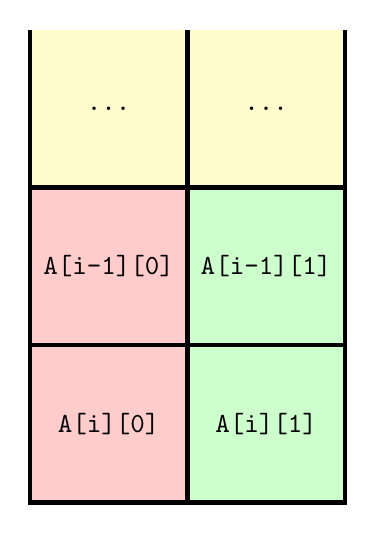
\begin{tikzpicture}[draw=black, ultra thick, x=\Size,y=\Size,
    node distance=2cm,
    c/.style={    inner sep=0pt,
    text width=\Size, 
    minimum size=\Size,
    % draw=black,
    fill=yellow!20,
    align=center,
 append after command={% <= for the border
        \pgfextra{%
            \begin{pgfinterruptpath}\begin{pgfonlayer}{foreground}
            \draw[black, ultra thick] let \p1=($(\tikzlastnode.north east)+(-0.5\pgflinewidth,-0.5\pgflinewidth)$),
                \p2=($(\tikzlastnode.north west)+(0.5\pgflinewidth,-0.5\pgflinewidth)$),
                \p3=($(\tikzlastnode.south west)+(0.5\pgflinewidth,0.5\pgflinewidth)$),
                \p4=($(\tikzlastnode.south east)+(-0.5\pgflinewidth,0.5\pgflinewidth)$) in
                (\p1) -- (\p4) -- (\p3) -- (\p2);
            \end{pgfonlayer}\end{pgfinterruptpath}
        }
    }},
]
\pgfmathsetmacro{\col}{1}; \pgfmathsetmacro{\row}{1};
\node [c] at ($(\col,-\row)-(0.5,0.5)$) { \texttt{... }};
\pgfmathsetmacro{\col}{1}; \pgfmathsetmacro{\row}{2};
\node [Square,draw=black, ultra thick,fill=red!20] at ($(\col,-\row)-(0.5,0.5)$) { \texttt{A[i-1][0] }};
\pgfmathsetmacro{\col}{1}; \pgfmathsetmacro{\row}{3};
\node [Square,draw=black, ultra thick,fill=red!20] at ($(\col,-\row)-(0.5,0.5)$) { \texttt{A[i][0] }};
\pgfmathsetmacro{\col}{2}; \pgfmathsetmacro{\row}{1};
\node [c] at ($(\col,-\row)-(0.5,0.5)$) { \texttt{... }};
\pgfmathsetmacro{\col}{2}; \pgfmathsetmacro{\row}{2};
\node [Square,draw=black, ultra thick,fill=green!20] at ($(\col,-\row)-(0.5,0.5)$) { \texttt{A[i-1][1] }};
\pgfmathsetmacro{\col}{2}; \pgfmathsetmacro{\row}{3};
\node [Square,draw=black, ultra thick,fill=green!20] at ($(\col,-\row)-(0.5,0.5)$) { \texttt{A[i][1] }};
\end{tikzpicture}

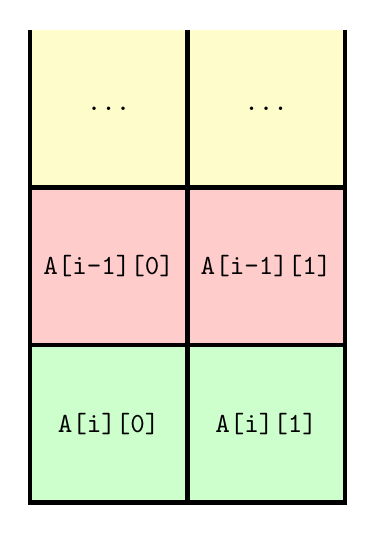
\begin{tikzpicture}[draw=black, ultra thick, x=\Size,y=\Size,
    node distance=2cm,
    c/.style={    inner sep=0pt,
    text width=\Size, 
    minimum size=\Size,
    % draw=black,
    fill=yellow!20,
    align=center,
 append after command={% <= for the border
        \pgfextra{%
            \begin{pgfinterruptpath}\begin{pgfonlayer}{foreground}
            \draw[black, ultra thick] let \p1=($(\tikzlastnode.north east)+(-0.5\pgflinewidth,-0.5\pgflinewidth)$),
                \p2=($(\tikzlastnode.north west)+(0.5\pgflinewidth,-0.5\pgflinewidth)$),
                \p3=($(\tikzlastnode.south west)+(0.5\pgflinewidth,0.5\pgflinewidth)$),
                \p4=($(\tikzlastnode.south east)+(-0.5\pgflinewidth,0.5\pgflinewidth)$) in
                (\p1) -- (\p4) -- (\p3) -- (\p2);
            \end{pgfonlayer}\end{pgfinterruptpath}
        }
    }},
]
\pgfmathsetmacro{\col}{1}; \pgfmathsetmacro{\row}{1};
\node [c] at ($(\col,-\row)-(0.5,0.5)$) { \texttt{... }};
\pgfmathsetmacro{\col}{1}; \pgfmathsetmacro{\row}{2};
\node [Square,draw=black, ultra thick,fill=red!20] at ($(\col,-\row)-(0.5,0.5)$) { \texttt{A[i-1][0] }};
\pgfmathsetmacro{\col}{1}; \pgfmathsetmacro{\row}{3};
\node [Square,draw=black, ultra thick,fill=green!20] at ($(\col,-\row)-(0.5,0.5)$) { \texttt{A[i][0] }};
\pgfmathsetmacro{\col}{2}; \pgfmathsetmacro{\row}{1};
\node [c] at ($(\col,-\row)-(0.5,0.5)$) { \texttt{... }};
\pgfmathsetmacro{\col}{2}; \pgfmathsetmacro{\row}{2};
\node [Square,draw=black, ultra thick,fill=red!20] at ($(\col,-\row)-(0.5,0.5)$) { \texttt{A[i-1][1] }};
\pgfmathsetmacro{\col}{2}; \pgfmathsetmacro{\row}{3};
\node [Square,draw=black, ultra thick,fill=green!20] at ($(\col,-\row)-(0.5,0.5)$) { \texttt{A[i][1] }};
\end{tikzpicture}


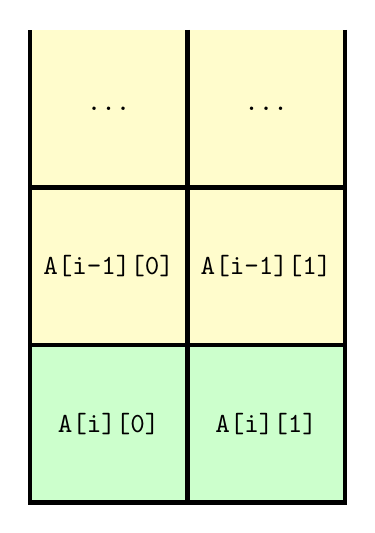
\begin{tikzpicture}[draw=black, ultra thick, x=\Size,y=\Size,
    node distance=2cm,
    c/.style={    inner sep=0pt,
    text width=\Size, 
    minimum size=\Size,
    % draw=black,
    fill=yellow!20,
    align=center,
 append after command={% <= for the border
        \pgfextra{%
            \begin{pgfinterruptpath}\begin{pgfonlayer}{foreground}
            \draw[black, ultra thick] let \p1=($(\tikzlastnode.north east)+(-0.5\pgflinewidth,-0.5\pgflinewidth)$),
                \p2=($(\tikzlastnode.north west)+(0.5\pgflinewidth,-0.5\pgflinewidth)$),
                \p3=($(\tikzlastnode.south west)+(0.5\pgflinewidth,0.5\pgflinewidth)$),
                \p4=($(\tikzlastnode.south east)+(-0.5\pgflinewidth,0.5\pgflinewidth)$) in
                (\p1) -- (\p4) -- (\p3) -- (\p2);
            \end{pgfonlayer}\end{pgfinterruptpath}
        }
    }},
]
\pgfmathsetmacro{\col}{1}; \pgfmathsetmacro{\row}{1};
\node [c] at ($(\col,-\row)-(0.5,0.5)$) { \texttt{... }};
\pgfmathsetmacro{\col}{1}; \pgfmathsetmacro{\row}{2};
\node [Square,draw=black, ultra thick] at ($(\col,-\row)-(0.5,0.5)$) { \texttt{A[i-1][0] }};
\pgfmathsetmacro{\col}{1}; \pgfmathsetmacro{\row}{3};
\node [Square,draw=black, ultra thick,fill=green!20] at ($(\col,-\row)-(0.5,0.5)$) { \texttt{A[i][0] }};
\pgfmathsetmacro{\col}{2}; \pgfmathsetmacro{\row}{1};
\node [c] at ($(\col,-\row)-(0.5,0.5)$) { \texttt{... }};
\pgfmathsetmacro{\col}{2}; \pgfmathsetmacro{\row}{2};
\node [Square,draw=black, ultra thick] at ($(\col,-\row)-(0.5,0.5)$) { \texttt{A[i-1][1] }};
\pgfmathsetmacro{\col}{2}; \pgfmathsetmacro{\row}{3};
\node [Square,draw=black, ultra thick,fill=green!20] at ($(\col,-\row)-(0.5,0.5)$) { \texttt{A[i][1] }};
\end{tikzpicture}

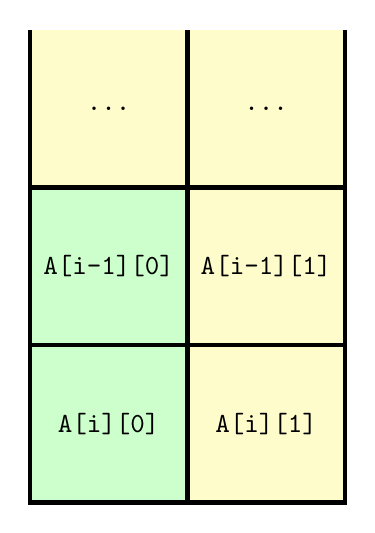
\begin{tikzpicture}[draw=black, ultra thick, x=\Size,y=\Size,
    node distance=2cm,
    c/.style={    inner sep=0pt,
    text width=\Size, 
    minimum size=\Size,
    % draw=black,
    fill=yellow!20,
    align=center,
 append after command={% <= for the border
        \pgfextra{%
            \begin{pgfinterruptpath}\begin{pgfonlayer}{foreground}
            \draw[black, ultra thick] let \p1=($(\tikzlastnode.north east)+(-0.5\pgflinewidth,-0.5\pgflinewidth)$),
                \p2=($(\tikzlastnode.north west)+(0.5\pgflinewidth,-0.5\pgflinewidth)$),
                \p3=($(\tikzlastnode.south west)+(0.5\pgflinewidth,0.5\pgflinewidth)$),
                \p4=($(\tikzlastnode.south east)+(-0.5\pgflinewidth,0.5\pgflinewidth)$) in
                (\p1) -- (\p4) -- (\p3) -- (\p2);
            \end{pgfonlayer}\end{pgfinterruptpath}
        }
    }},
]
\pgfmathsetmacro{\col}{1}; \pgfmathsetmacro{\row}{1};
\node [c] at ($(\col,-\row)-(0.5,0.5)$) { \texttt{... }};
\pgfmathsetmacro{\col}{1}; \pgfmathsetmacro{\row}{2};
\node [Square,draw=black, ultra thick,fill=green!20] at ($(\col,-\row)-(0.5,0.5)$) { \texttt{A[i-1][0] }};
\pgfmathsetmacro{\col}{1}; \pgfmathsetmacro{\row}{3};
\node [Square,draw=black, ultra thick,fill=green!20] at ($(\col,-\row)-(0.5,0.5)$) { \texttt{A[i][0] }};
\pgfmathsetmacro{\col}{2}; \pgfmathsetmacro{\row}{1};
\node [c] at ($(\col,-\row)-(0.5,0.5)$) { \texttt{... }};
\pgfmathsetmacro{\col}{2}; \pgfmathsetmacro{\row}{2};
\node [Square,draw=black, ultra thick] at ($(\col,-\row)-(0.5,0.5)$) { \texttt{A[i-1][1] }};
\pgfmathsetmacro{\col}{2}; \pgfmathsetmacro{\row}{3};
\node [Square,draw=black, ultra thick] at ($(\col,-\row)-(0.5,0.5)$) { \texttt{A[i][1] }};
\end{tikzpicture}


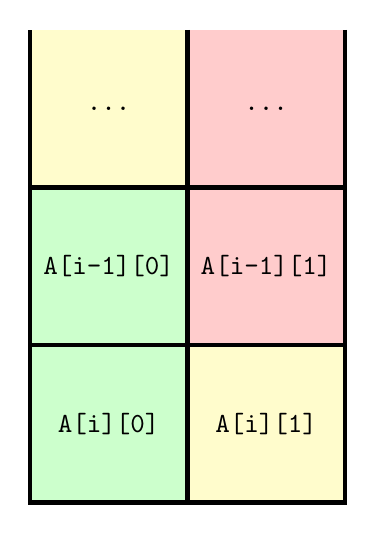
\begin{tikzpicture}[draw=black, ultra thick, x=\Size,y=\Size,
    node distance=2cm,
    c/.style={    inner sep=0pt,
    text width=\Size, 
    minimum size=\Size,
    % draw=black,
    fill=yellow!20,
    align=center,
 append after command={% <= for the border
        \pgfextra{%
            \begin{pgfinterruptpath}\begin{pgfonlayer}{foreground}
            \draw[black, ultra thick] let \p1=($(\tikzlastnode.north east)+(-0.5\pgflinewidth,-0.5\pgflinewidth)$),
                \p2=($(\tikzlastnode.north west)+(0.5\pgflinewidth,-0.5\pgflinewidth)$),
                \p3=($(\tikzlastnode.south west)+(0.5\pgflinewidth,0.5\pgflinewidth)$),
                \p4=($(\tikzlastnode.south east)+(-0.5\pgflinewidth,0.5\pgflinewidth)$) in
                (\p1) -- (\p4) -- (\p3) -- (\p2);
            \end{pgfonlayer}\end{pgfinterruptpath}
        }
    }},
]
\pgfmathsetmacro{\col}{1}; \pgfmathsetmacro{\row}{1};
\node [c] at ($(\col,-\row)-(0.5,0.5)$) { \texttt{... }};
\pgfmathsetmacro{\col}{1}; \pgfmathsetmacro{\row}{2};
\node [Square,draw=black, ultra thick,fill=green!20] at ($(\col,-\row)-(0.5,0.5)$) { \texttt{A[i-1][0] }};
\pgfmathsetmacro{\col}{1}; \pgfmathsetmacro{\row}{3};
\node [Square,draw=black, ultra thick,fill=green!20] at ($(\col,-\row)-(0.5,0.5)$) { \texttt{A[i][0] }};
\pgfmathsetmacro{\col}{2}; \pgfmathsetmacro{\row}{1};
\node [c,fill=red!20] at ($(\col,-\row)-(0.5,0.5)$) { \texttt{... }};
\pgfmathsetmacro{\col}{2}; \pgfmathsetmacro{\row}{2};
\node [Square,draw=black, ultra thick,fill=red!20] at ($(\col,-\row)-(0.5,0.5)$) { \texttt{A[i-1][1] }};
\pgfmathsetmacro{\col}{2}; \pgfmathsetmacro{\row}{3};
\node [Square,draw=black, ultra thick] at ($(\col,-\row)-(0.5,0.5)$) { \texttt{A[i][1] }};
\end{tikzpicture}


\end{document}

% 3 2
% 2 2
% 3 3
% 2 1
